\documentclass[12pt]{article}
\usepackage[utf8]{inputenc}
\usepackage{array}
\usepackage{graphicx}
\usepackage{xcolor}
\title{Development Plan}
\author{ SWFRENG 3XA3 }

\begin{document}

\maketitle
\noindent
Group 30
\newline
Team Name: Team 30
\newline
Team Member No.1: Alan Yin
\newline
Team Member No.2: Huajie Zhu
\newline
Team Member No.3: Junni Pan

\section{Team Meeting Plan}
Basically, we are going to meet three times every week, including two lab times and another one will be at mills library on weekend. Our member Alan will chair every meeting, inform us about the topic for a meeting and how can we prepare for it. Every member in the group needs to complete his own work before a meeting, and cooperates with other members during the meeting time. After the meeting, we need to review meeting's effectiveness and distribute new work to every one. For review every meeting's effectiveness, we will use a meeting agenda to help us.


\subsection*{Meeting Agenda}

\begin{figure}
\centering
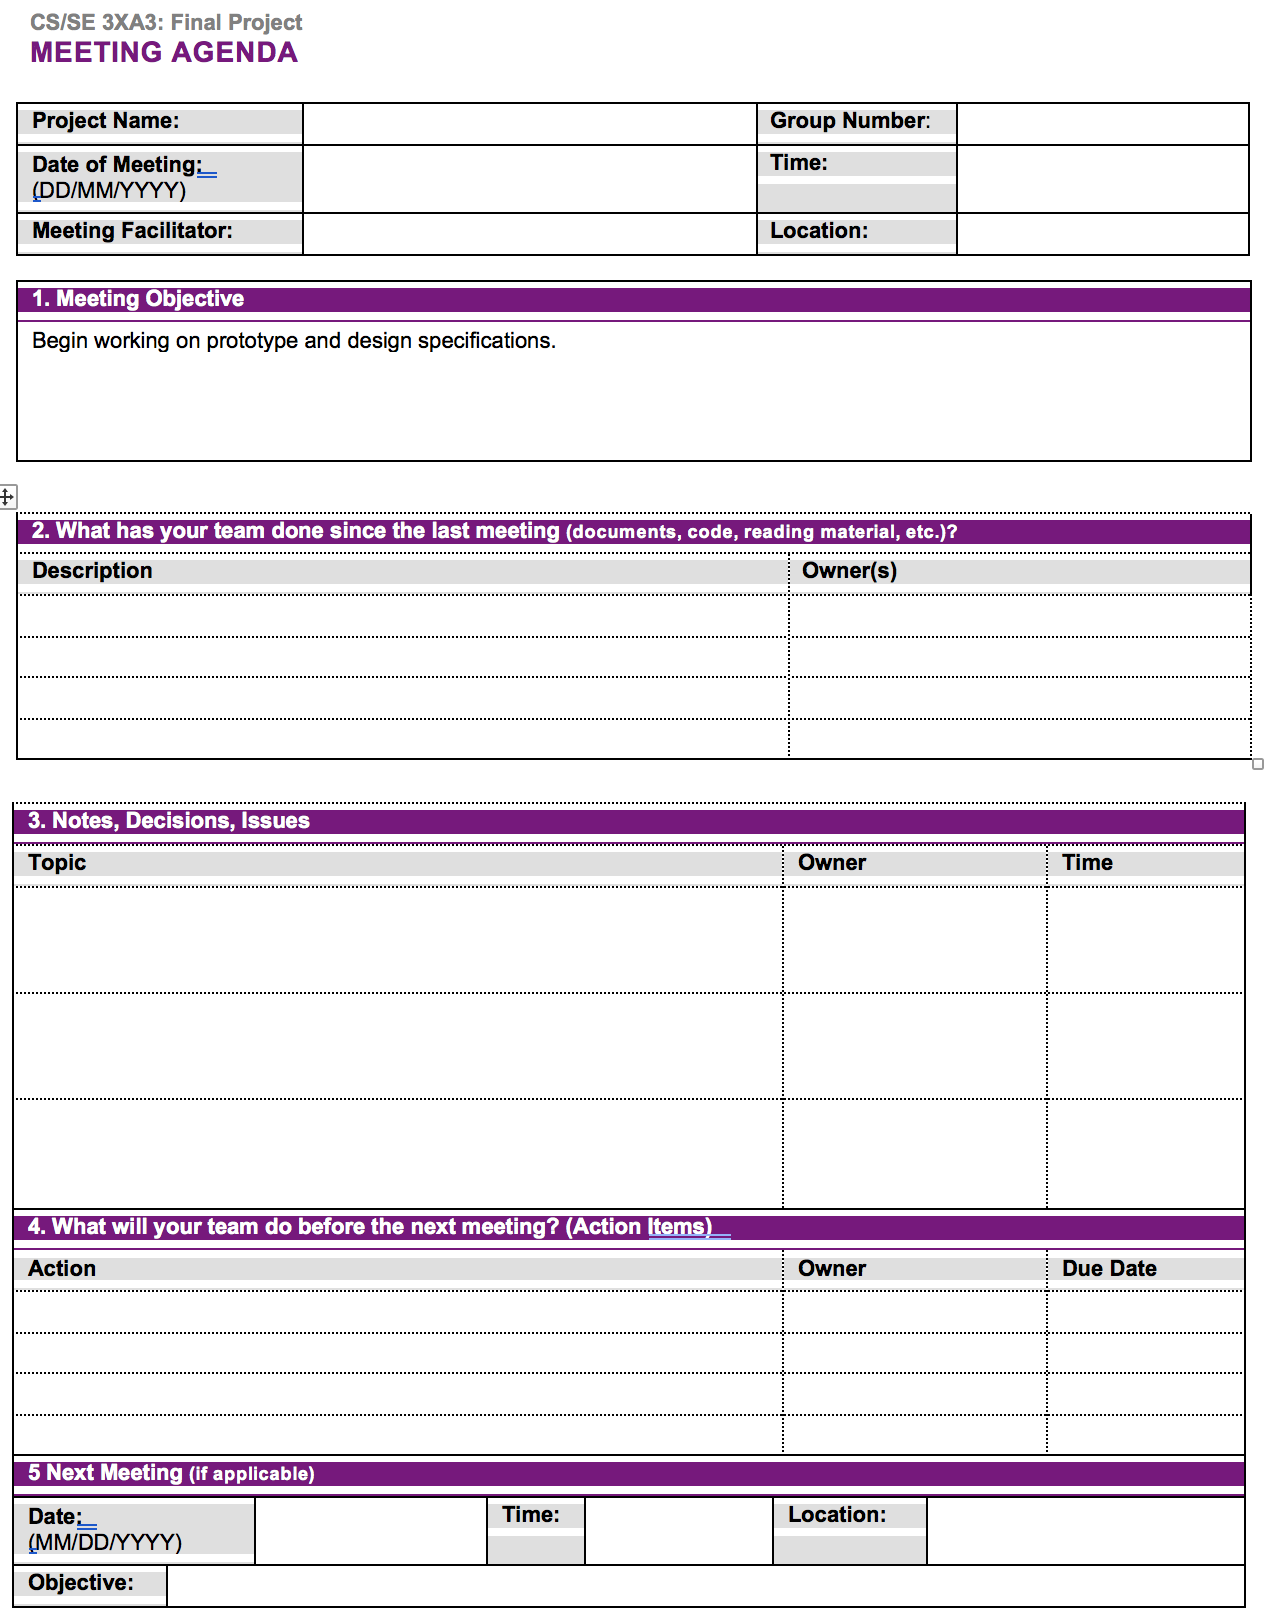
\includegraphics[width=15cm]{img/meetingAgenda.png}
\end{figure}


\newpage
\section{Communication Plan}
We will use WeChat to communicate with each other, and discuss about our project process. For file sharing and modification, we will make use of GitLab's features and its tools. We can also use text or email to contact each other.

\section{Team Member Roles}
\begin{tabular}{ | m{8em} | m{4.5cm}| m{4.5cm} | } 
\hline
Member Name & Position & Experts on \\
\hline
Alan Yin & Leader, Programmer & Git, Java \\ 
\hline
Huajie Zhu & Scribe, Tester & Documentation, Java  \\ 
\hline
Junni Pan & Scribe, Programmer & LaTeX, \color{red}{Slick2D}\\ 
\hline
\end{tabular}

\noindent
\newline
Alan is our team leader and programmer. He is going to manage every meeting and distribute work to us. He also need to handle Git and Java programming. Huajie is our team scribe and tester. He is going to record our meetings and update our documents. He also need to test our program. Junni is another scribe and programmer. He need to familiars with LaTex operations. He also should work on \color{red}{Slick2D}, and make it run well on our program\color{black}.

\section{Git Workflow Plan}
\begin{figure}
\centering
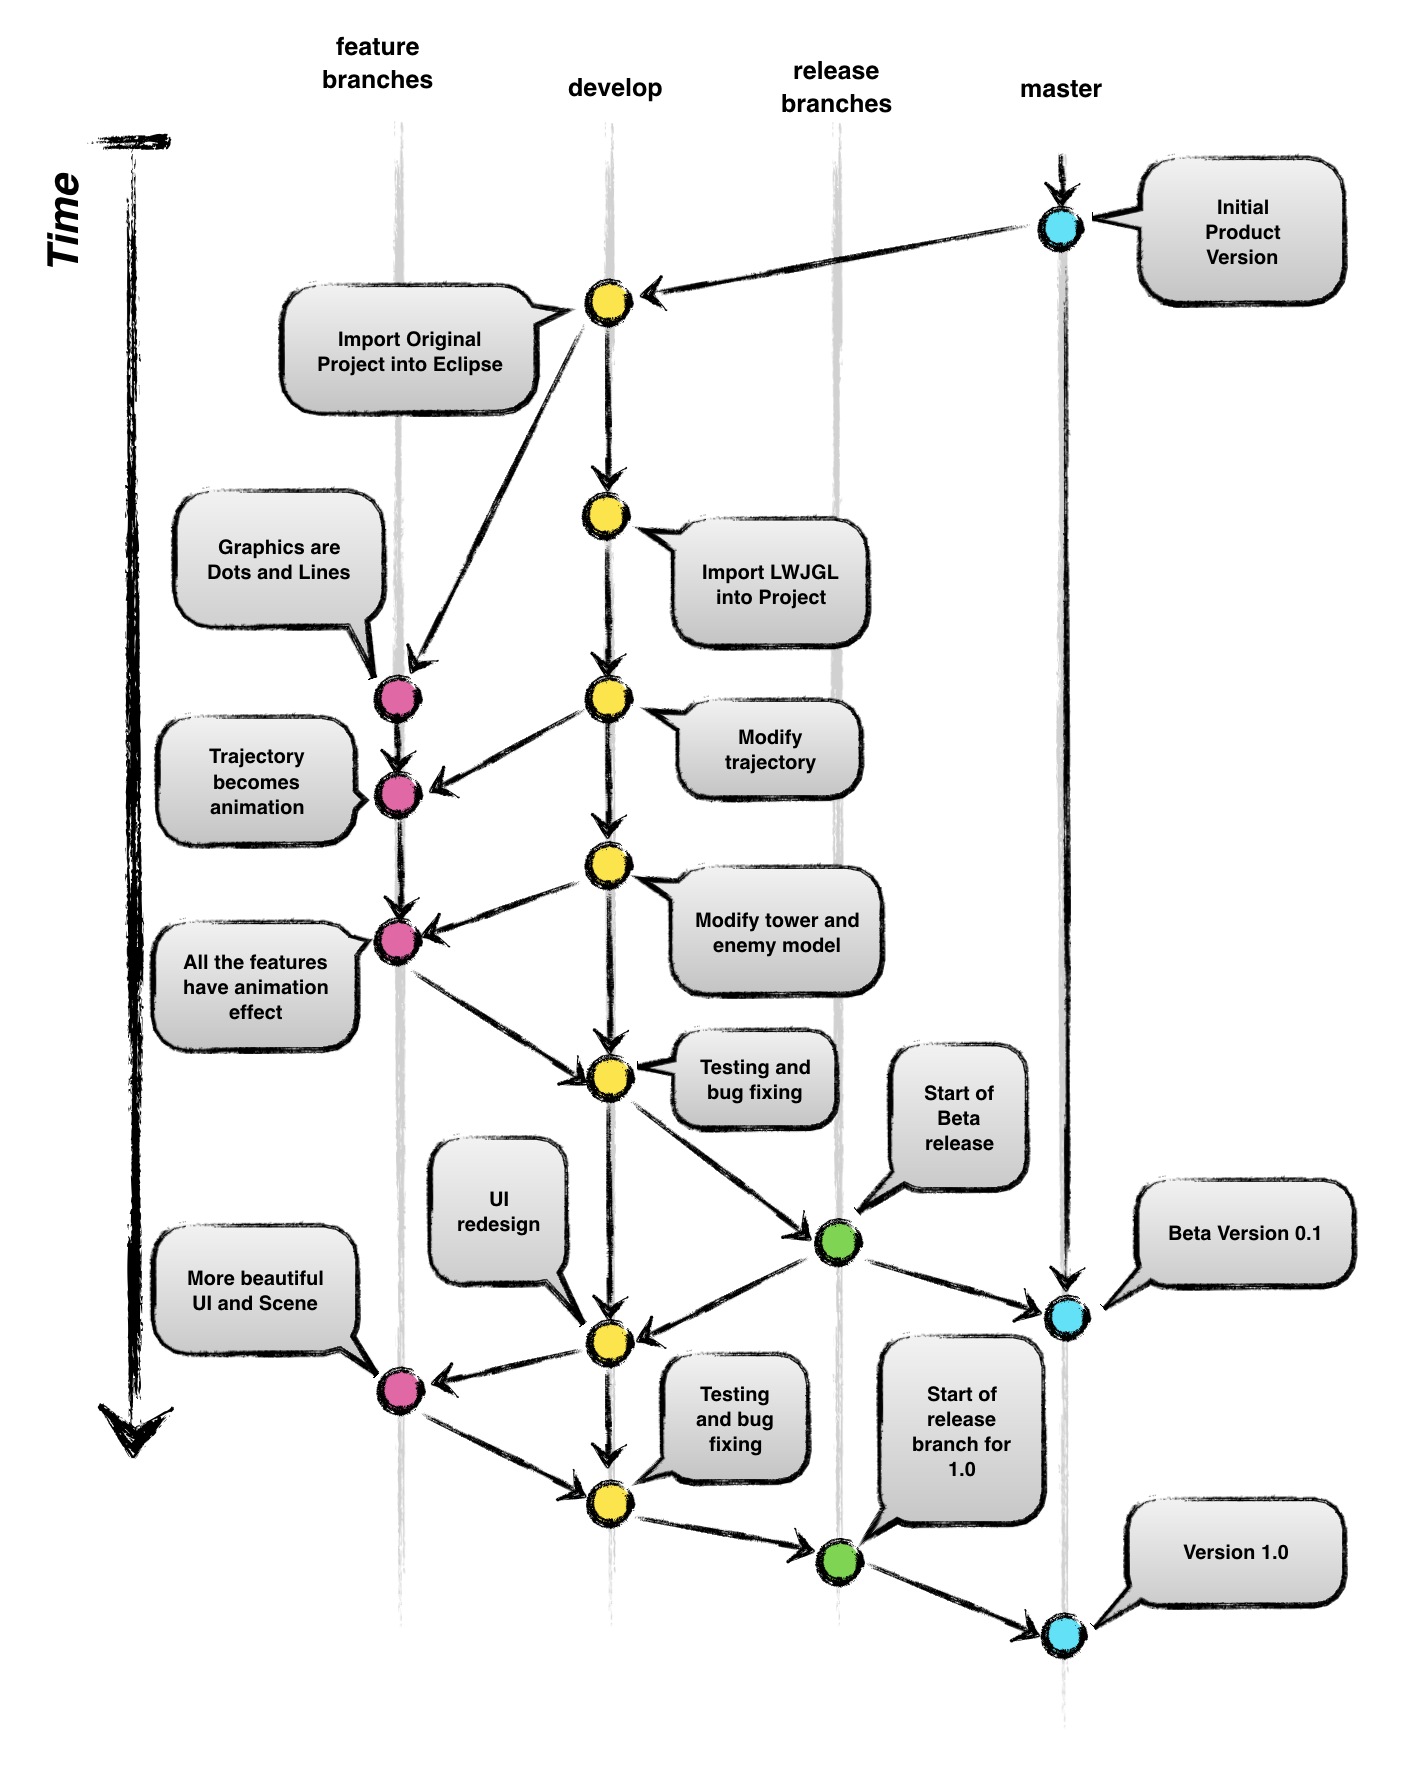
\includegraphics[width=16cm]{img/GitWorkflow.png}
\end{figure}
\newpage

\section{Proof of Concept Development Plan}
For our project, the most difficult part is to run the program with \color{red}Slick2D, which is a simplified version of OpenGL\color{black}. Because we want our game to have a beautiful graphic effect and lively animation. So the most important thing to proof is how well can we make the use of this \color{red}Slick2D\color{black}. The testing could be hard because no one is familiar with this library. It is not difficult to install but it may be difficult to combine with the current program. We want to demonstrate how much the game has improved compared with the current game, in order to do the proof of concept.

\section{Technology}
\begin{tabular}{ | m{12em} | m{6cm} | } 
\hline
Field & Technology \\
\hline
Programming Language & Java \\ 
\hline
IDE & Eclipse \\ 
\hline
Game Engine & \color{red}{Slick2D} \\ 
\hline
Testing Framework & Junit \\
\hline
Document Generation & Javadoc \\
\hline
\end{tabular}

\section{Coding Style}
Basically, we need to make our code neat, simple and elegant. We can follow the Google Java Style Guide and make every member use the same style to code.

\section{Project Schedule}
\begin{figure}
\centering
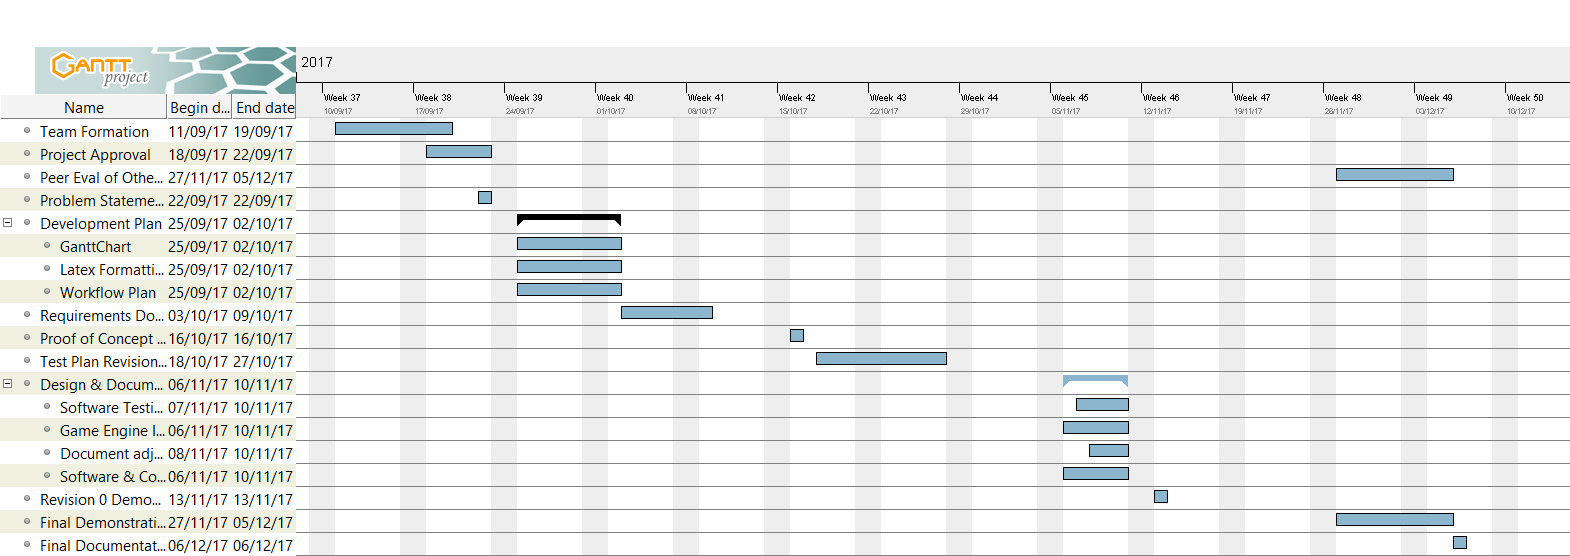
\includegraphics[width=16cm]{img/gantt1.png}
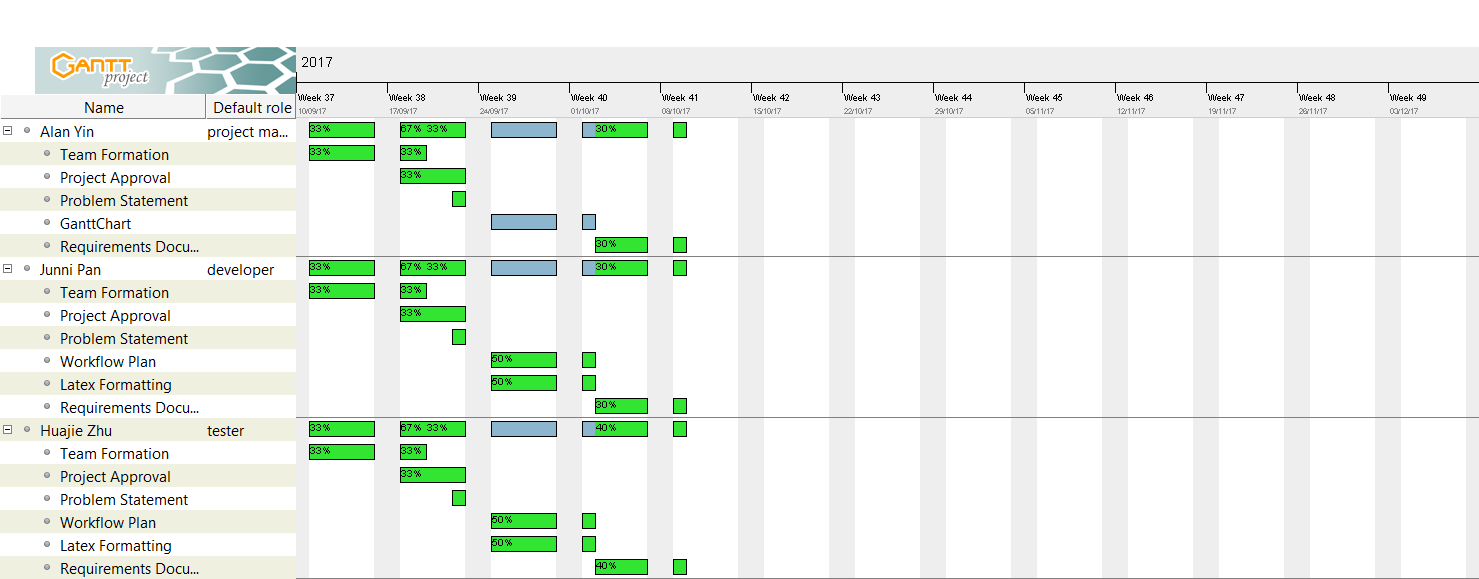
\includegraphics[width=16cm]{img/gantt2.png}
\end{figure}
\newpage

\section{Project Review}
\color{red}
The Tower Defense Project is a re-implementation on an open source project. It is aimed to provide us a chance to experience the software development life cycle. During this project, we are able to practise writing formal documentations, group communication, and programming skills at the same time. Our group followed the meeting schedule, and divided all the works reasonably based on the skills of each member. We were a bit behind the development plan during proof of concept demo, but we managed to catch up in the later portion of this project. Overall, the schedules are followed and the all the requirements are accomplished.
\color{black}


\end{document}
